\clearpage
\subsection{Login}
The application designed in this report will include a login feature. Each user will need a username and password to login.
A user can be assigned one or more of these roles:

\begin{itemize}
    \item Student
    \item Teacher
    \item Administrator
\end{itemize}

\noindent
By using a login feature the application will provide a way to keep track of the data for each user as well as making sure certain features only is accessed by specific roles such as administrators being the only ones to provide and change login information. A database will be used to store the login information and this will be further described in \textnameref{section:database_design}.
\newline\newline
The login screen will also feature an option to save credentials making it easier to log in next time when using the application.
\Figureref{fig:login_draft} shows a draft of what the login screen look like, with the boxes for user input, saving credentials and login easily visible.

\begin{figure}[H]
    \centering
    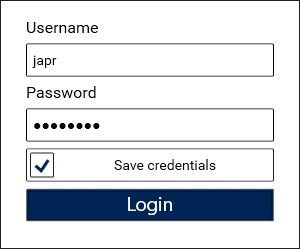
\includegraphics[width=0.35\textwidth]{figures/LoginDraft.png}
    \caption{Draft of Login screen}
    \label{fig:login_draft}
\end{figure}
